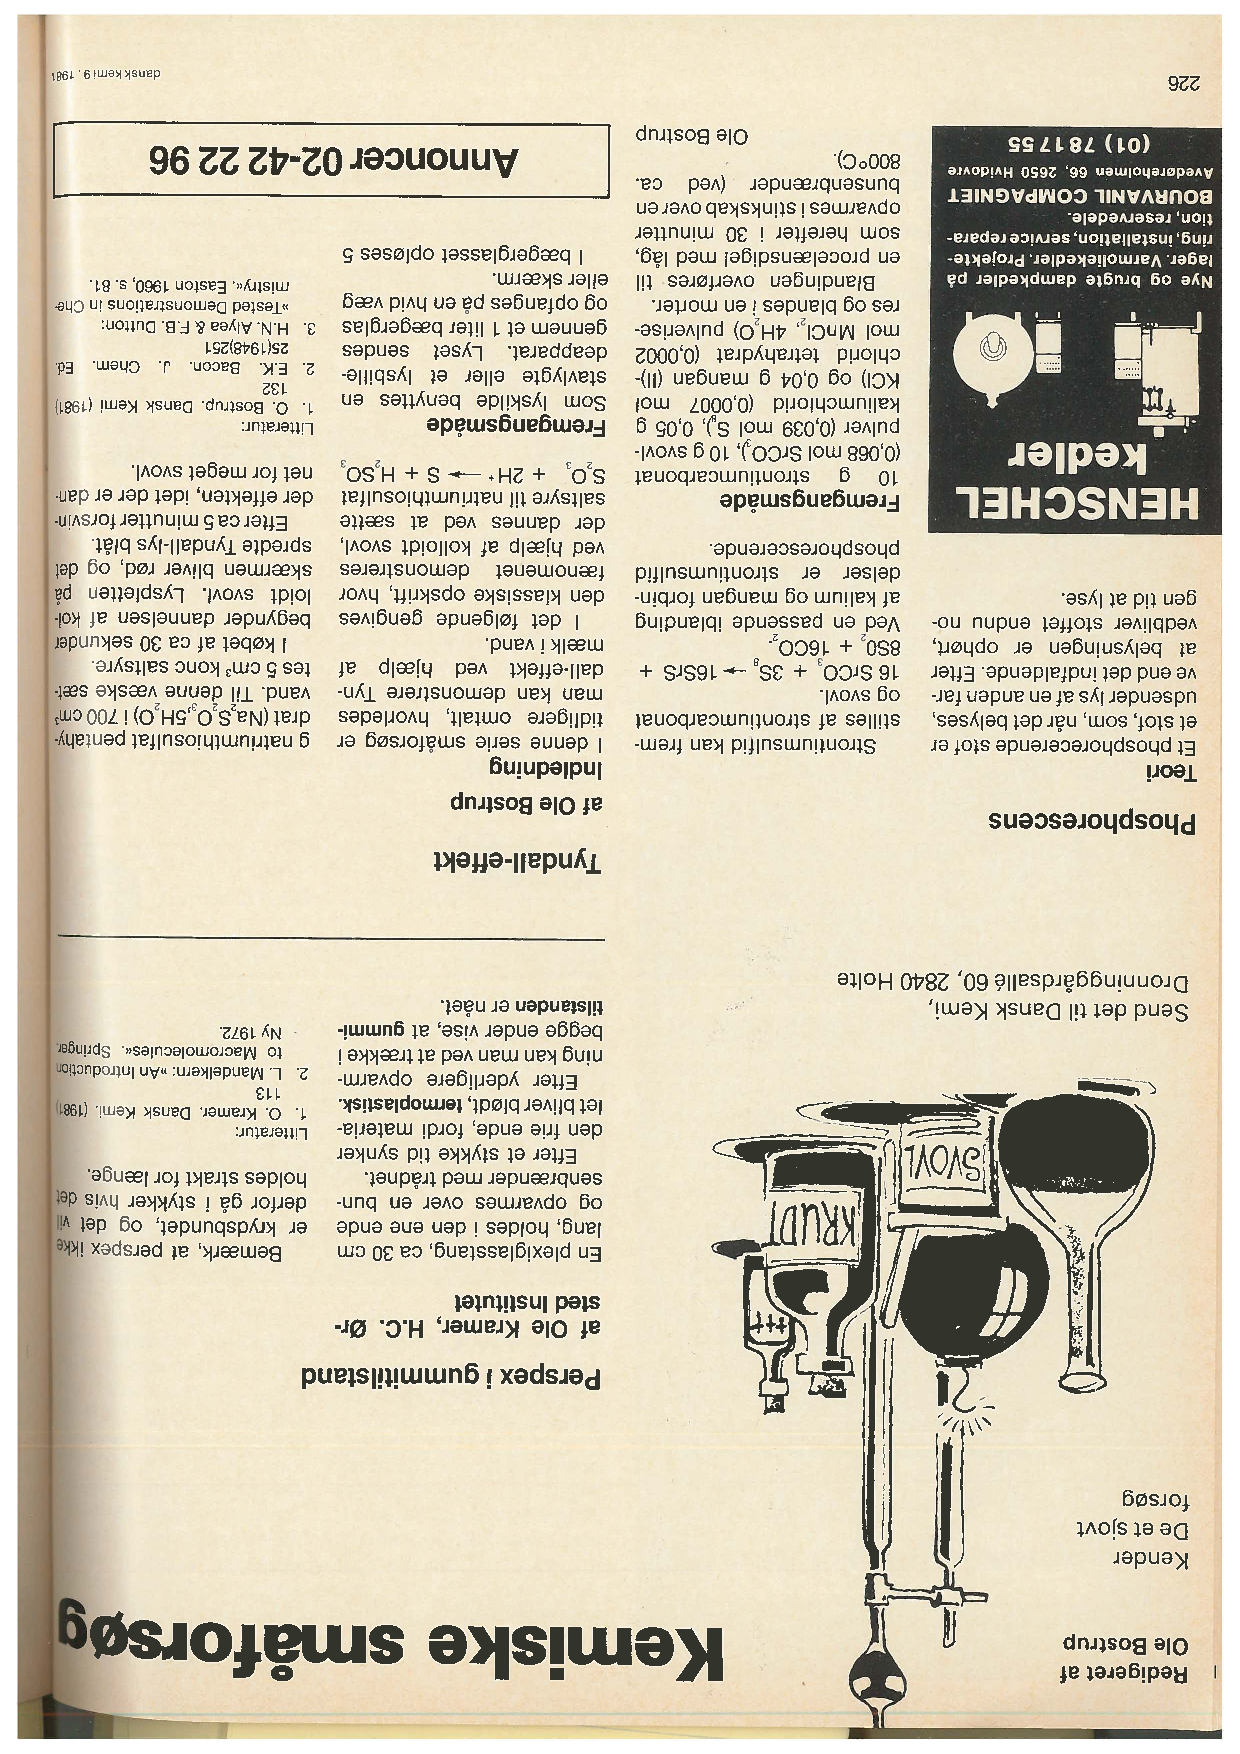
\includepdf[pages=-]{pdfs/1981-62-9-226.pdf}
\emne{Tyndall-effekt}
\danskkemi{Dansk Kemi 62, 9, 1981, p. 226}
\forfatter{Ole Bostrup}

\deloverskrift{Indledning}
I denne serie småforsøg er tidligere omtalt, hvorledes man kan
demonstrere Tyndall-effekt ved hjælp af mælk i vand.
I det følgende gengives den klassiske opskrift, hvor fænomenet
demonstreres ved hjælp af kolloidt svovl, der dannes ved at sætte
saltsyre til natriumthiosulfat
\ch{S2O3 + 2H+ -> S + H2SO3}

\deloverskrift{Fremgangsmåde}
Som lyskilde benyttes en stavlygte eller et lysbilledeapparat. Lyset
sendes gennem et 1 liter bægerglas og opfanges på en hvid væg eller
skærm.
I bægerglasset opløses 5 g natriumthiosulfat pentahydrat
(\ch{Na2S2O3 , 5 H2O}) i 700 cm3 vand. Til dene væske sættes 5 cm3
konc saltsyre.
I købet af ca 30 sekunder begynder dannelsen af kolloidt svovl.
Lyspletten på skærmen bliver rød, og det spredte Tyndall-lys blåt.
Efter ca 5 minutter forsvinder effekten, idet der er dannet for
meget svovl.

Litteratur:
1. O. Bostrup. Dansk Kemi (1981) 132
2. E.K. Bacon. J.Chem.Ed. 25(1948)251
3. H.N. Alyea \& F.B. Dutton: "Tested Demonstrations in Chemistry".
Easton 1960, s. 81.
